
\subsection{Función de Wood}

\subsubsection{Vector predefinido}

En la figura \ref{fig:wood} se muestran los resultados de cada iteración obtenidos por la función de Wood partiendo del vector de la ecuación \ref{eq:wood_vector}.

\begin{figure}[H]
    \centering
    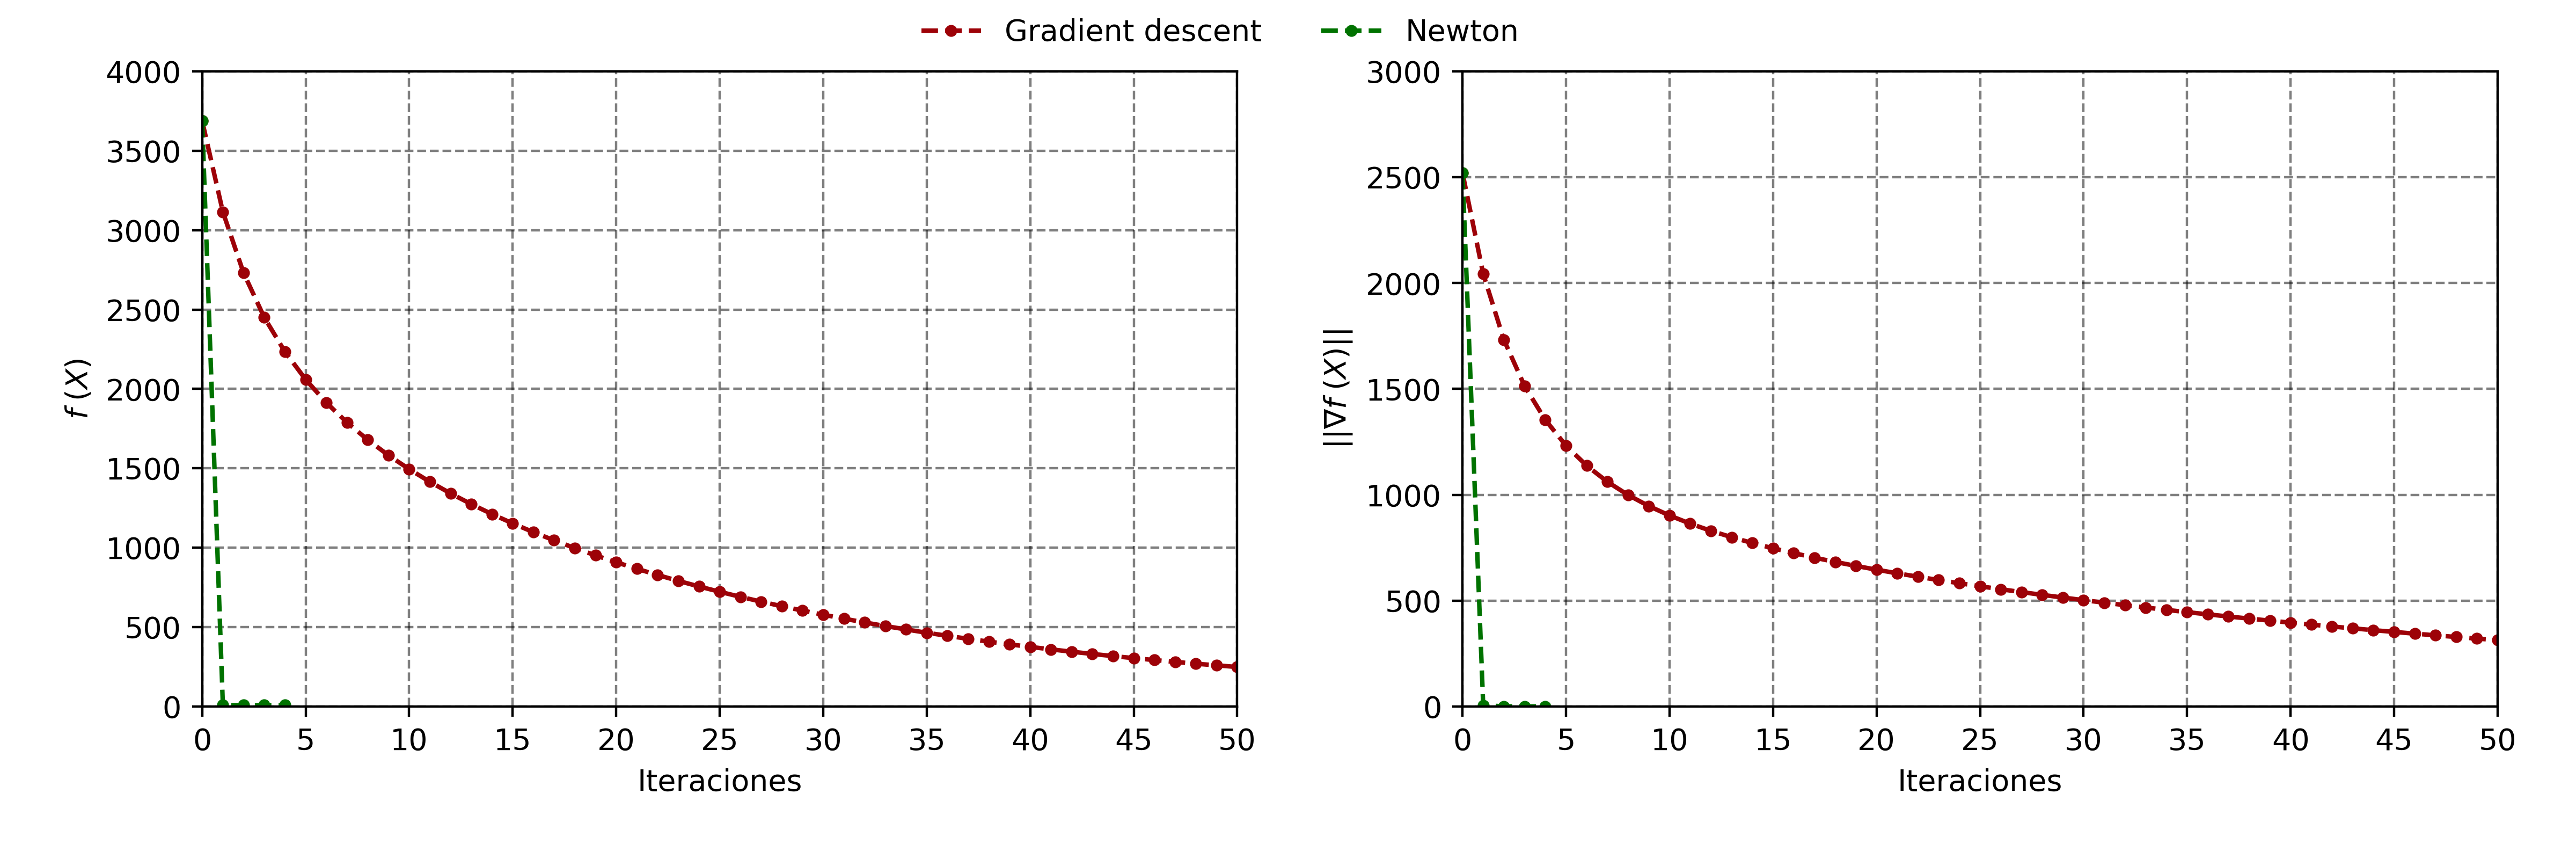
\includegraphics[width=12cm]{Graphics/Problema_2/wood_4_predefined.png}
    \caption{Iteraciones de los métodos del descenso del gradiente y de Newton aplicados a la función de Wood.}
    \label{fig:wood}
\end{figure}

En la tabla \ref{table:wood_predefined} se muestran los resultados de la primer y última iteracion para cada método.

\begin{table}[H]
    \centering
    \begin{tabular}{cccccc} \hline
        Método                 & Iteraciones & $f(x_0)$ & $f(x_n)$   & $\nabla f(x_0)$ & $\nabla f(x_n) $ \\ \hline
        Descenso del gradiente & 3094        & 0.000081 & $0.000002$ & $2520.7046$     & $0.019937$       \\
        Newton                 & 4           & 3688.000 & $7.876963$ & $2520.7046$     & $0.012216$       \\ \hline
    \end{tabular}
    \caption{Resultados de la primer y última iteración del método del descenso del gradiente y de Newton para la función de Rosembrock para dos dimensiones.}
    \label{table:wood_predefined}
\end{table}

\subsection{Vector aleatorio}

En la figura \ref{fig:wood_random} se muestran los resultados de cada iteración obtenidos por la función de Wood partiendo del vector de la ecuación \ref{eq:random_vector}.

\begin{figure}[H]
    \centering
    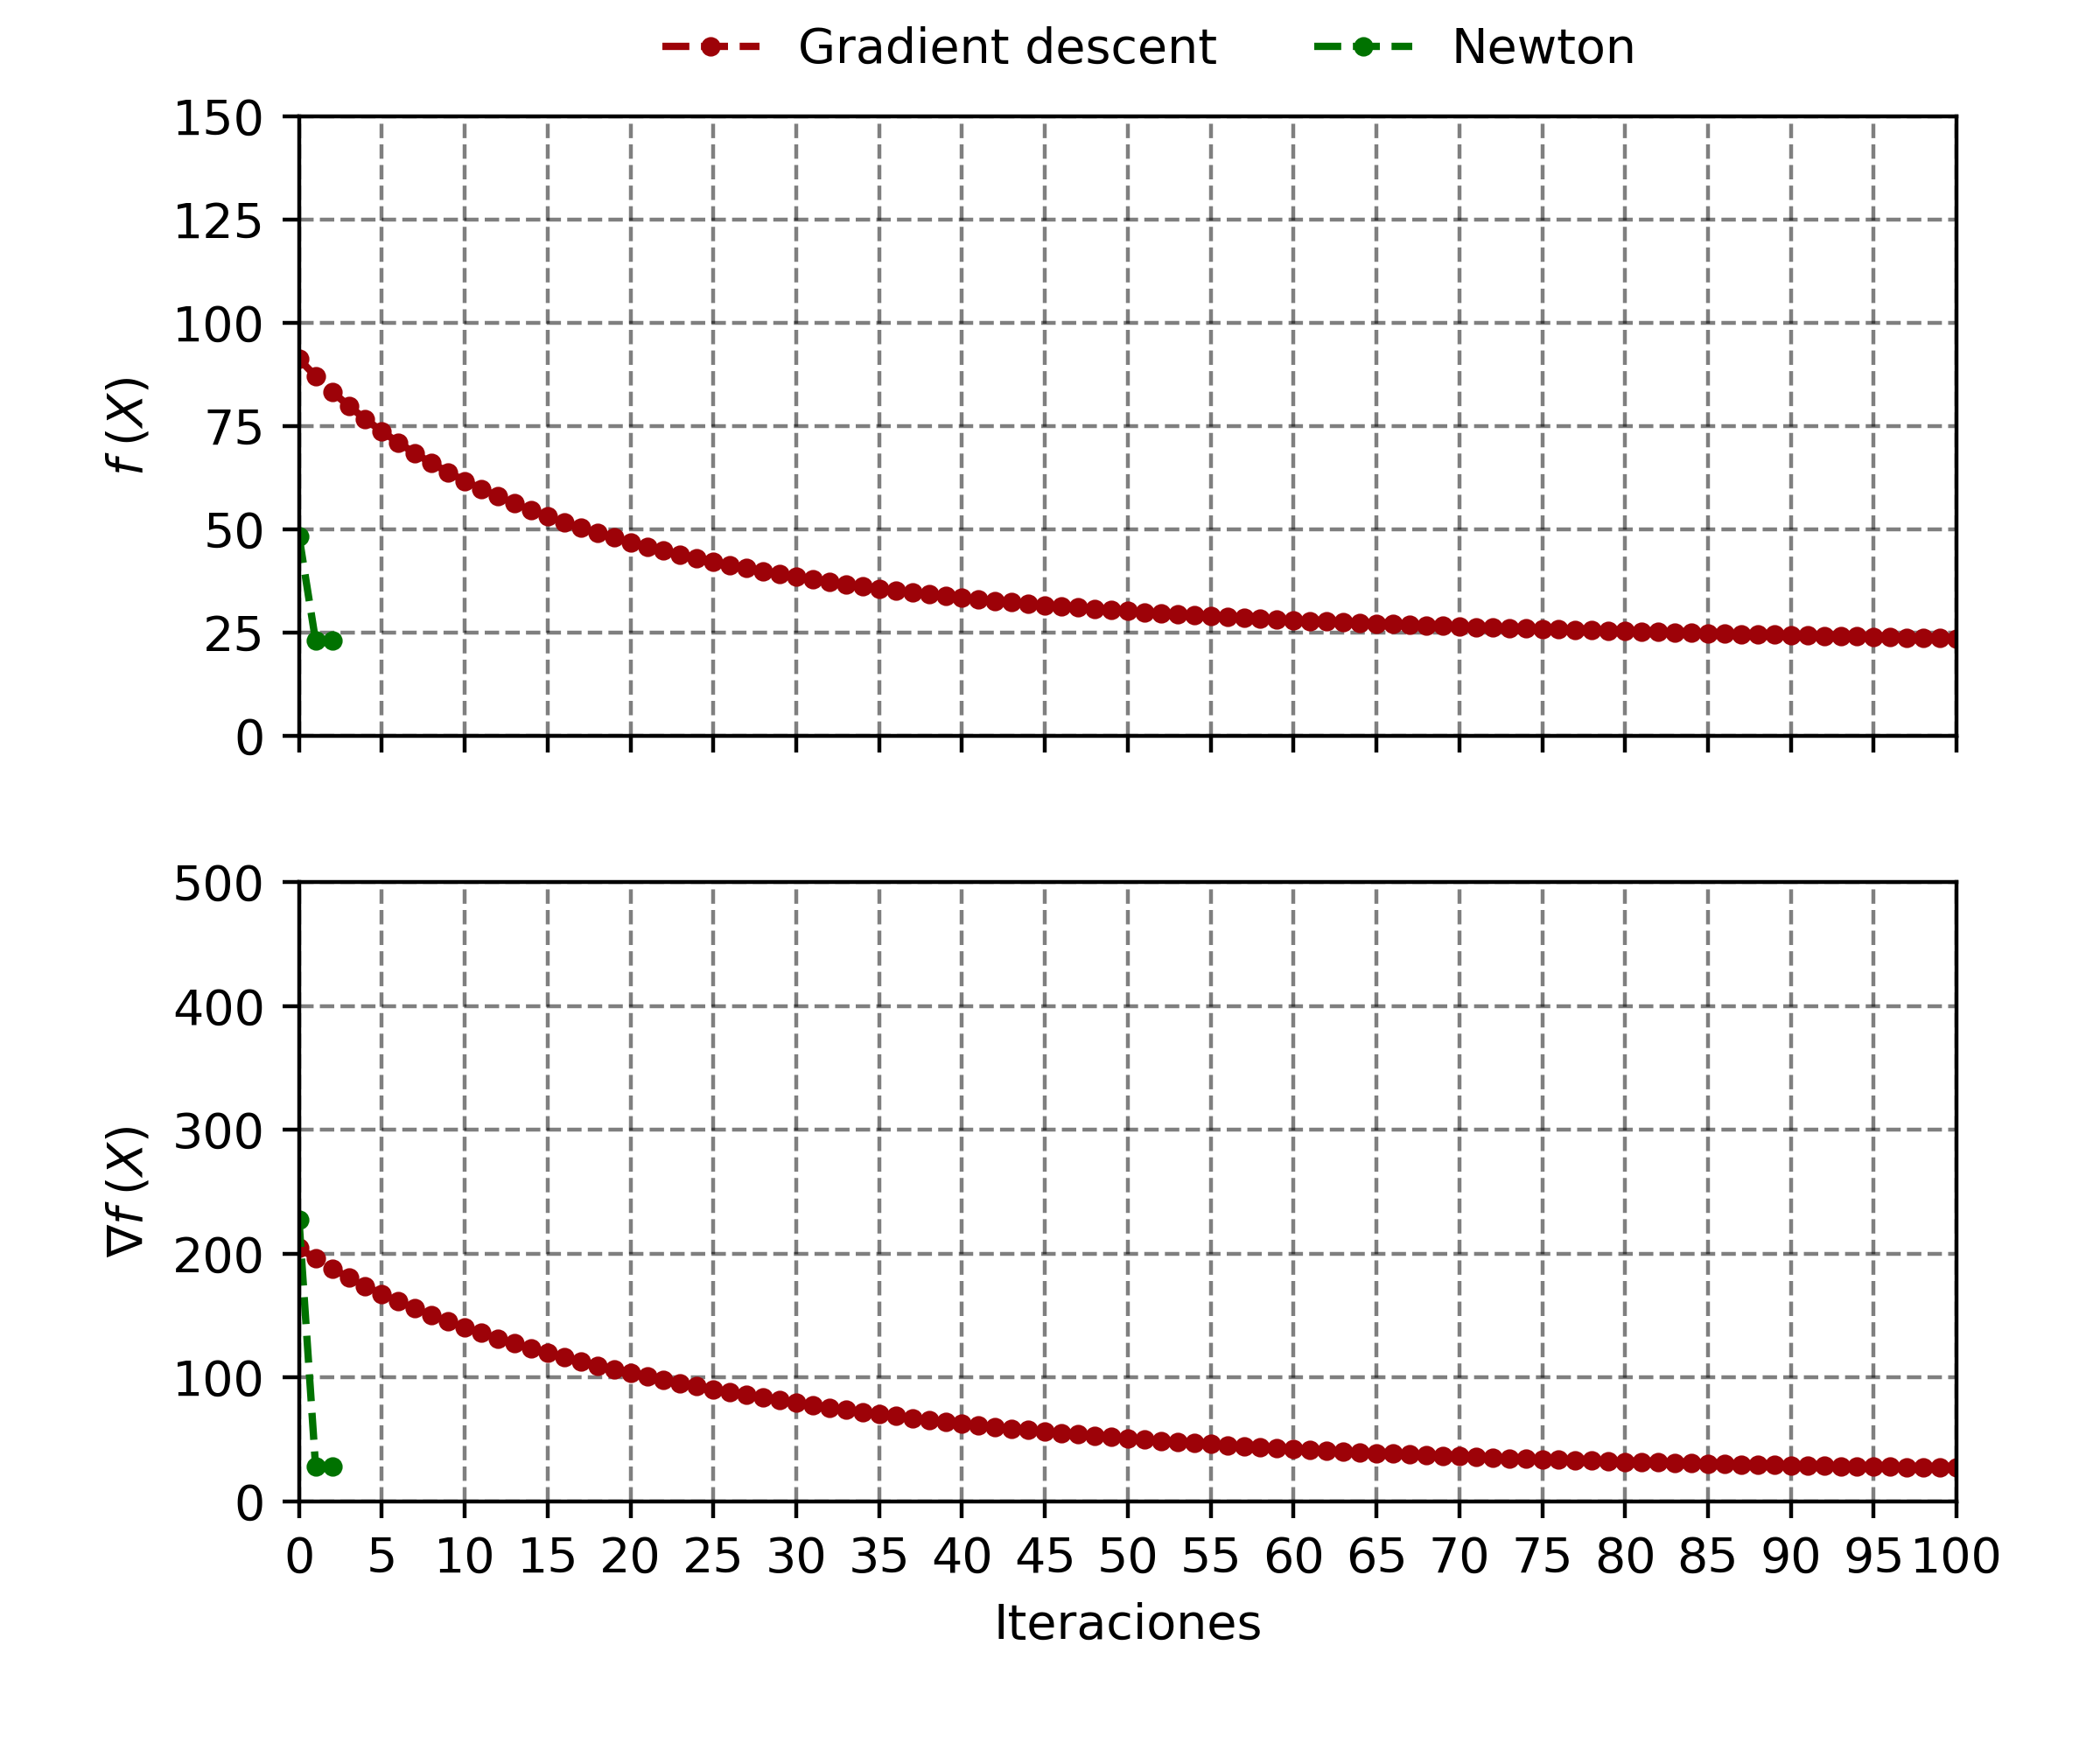
\includegraphics[width=12cm]{Graphics/Problema_2/wood_4_random.png}
    \caption{Iteraciones de los métodos del descenso del gradiente y de Newton aplicados a la función de Wood.}
    \label{fig:wood_random}
\end{figure}

En la tabla \ref{table:wood_random} se muestran los resultados de la primer y última iteracion para cada método.

\begin{table}[H]
    \centering
    \begin{tabular}{cccccc} \hline
        Método                 & Iteraciones & $f(x_0)$  & $f(x_n)$    & $\nabla f(x_0)$ & $\nabla f(x_n) $ \\ \hline
        Descenso del gradiente & 72711       & 91.214553 & $0.000278$  & $2520.7046$     & $0.019999$       \\
        Newton                 & 2           & 48.331395 & $23.010416$ & $227.054327$    & $28.070864$      \\ \hline
    \end{tabular}
    \caption{Resultados de la primer y última iteración del método del descenso del gradiente y de Newton para la función de Rosembrock para dos dimensiones.}
    \label{table:wood_random}
\end{table}

\subsubsection{Estadisticas}

Se ejecutaron los métodos de Newton y descenso del gradiente con 100 vectores aleatorios. Cada vector aleatorio esta creado en base a la ecuación \ref{eq:random_vector}.

\paragraph{Método de Newton}

En la figura se representa la distribución de los resultados obtenidos para $f(x^*)$ y $\nabla f(x^*)$.

\begin{table}[H]
    \centering
    \begin{tabular}{ccc} \hline
                 & $f(x)$   & $||\nabla f(x)||$ \\ \hline
        n        & 100      & 100               \\
        Media    & 14.12856 & 13.14793          \\
        $\sigma$ & 14.38304 & 16.05534          \\
        Mínimo   & 0        & 0                 \\
        Máximo   & 40.22492 & 72.09054          \\\hline
    \end{tabular}
    \caption{Media, desviación estandar, mínimo y máximo de los resultados aleatorios usando el método de Newton en la función de Wood.}
    \label{table:wood_100_random_newton}
\end{table}


\paragraph{Método del descenso de Gradiente}


\begin{table}[H]
    \centering
    \begin{tabular}{ccc} \hline
                 & $f(x)$     & $||\nabla f(x)||$ \\ \hline
        n        & 100.000000 & 100.000000        \\
        Media    & 0.315318   & 0.019965          \\
        $\sigma$ & 1.551148   & 0.000167          \\
        Mínimo   & 0.000278   & 0.019122          \\
        Máximo   & 7.876494   & 0.020000          \\ \hline
    \end{tabular}
    \caption{Media, desviación estandar, mínimo y máximo de los resultados aleatorios usando el método de Newton en la función de Wood.}
    \label{table:wood_100_random_gradient}
\end{table}
